\documentclass[final]{beamer}
\mode<presentation>
{
  \usetheme{I6pd2}
}
\graphicspath{{figures/}} % e.g. where you have your logos

\usepackage{times}
\usepackage{amsmath,amssymb}
\usepackage[english]{babel}
\usepackage[latin1]{inputenc}
\usepackage[orientation=portrait,size=a0,scale=1.25,debug]{beamerposter} 

\usepackage{epstopdf}


\title[Fancy Posters]{Reservoir Computing for Recurrent Neural Networks}
\author[Grezes \& Rosenberg]{Felix Grezes \{fgrezes@gc.cuny.edu\}\\
\vspace{5 mm}
advised by Pr. Andrew Rosenberg and Pr. Noemie Elhadad}
\institute[SLQC CUNY]{The Speech Lab at Queens College CUNY}
%\date{\today}
\begin{document}

\begin{columns}[t]
\begin{column}{.45\linewidth}

\bigskip

\begin{block}{\vspace{-9 mm} \LARGE Abstract}
\large
Historically, research has focused on {\em Recurrent Neural Networks} (RNNs)  because of their capacity to model dynamical system and/or their biological plausibility. However traditional neural network approaches, such has gradient descent, are either impossible or too slow to be applied successfully to RNNs.\\
The {\em Reservoir Computing} paradigm, by separating the optimization of the network layer from the output layer, attempts to solve these issues. Since 2001, it has proven itself to be fast and effective in a variety of applications.
\end{block}

\bigskip 

\begin{block}{\vspace{-13 mm} \LARGE The Reservoir Computing Paradigm}
\begin{figure}[t]
\fbox{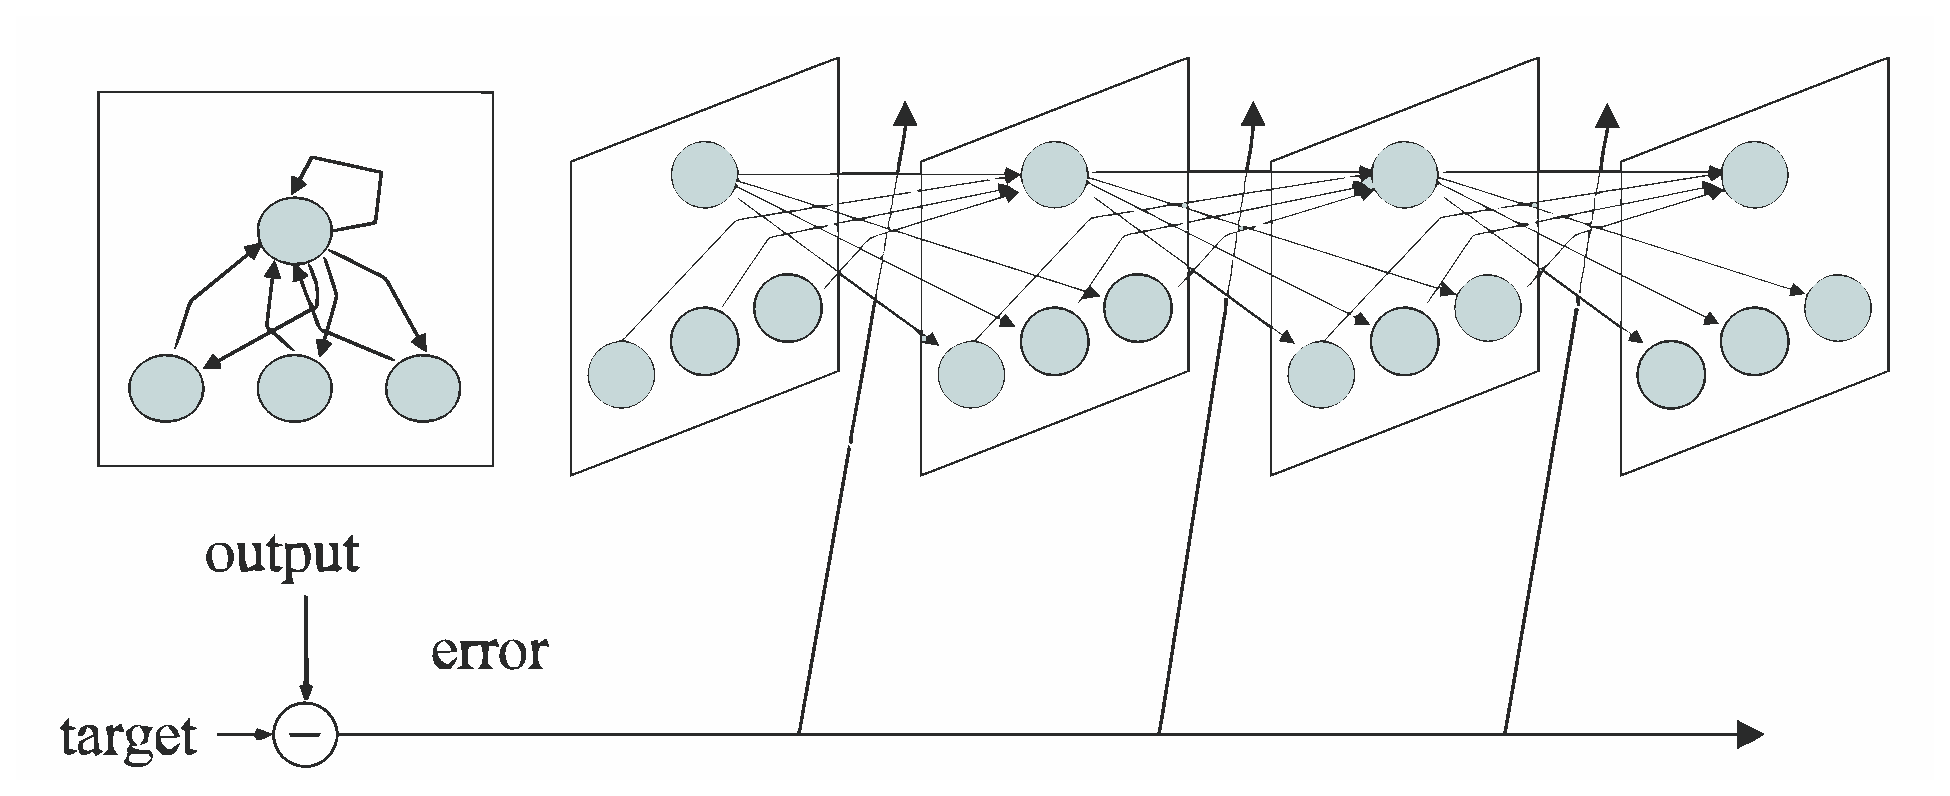
\includegraphics[width=0.9\linewidth]{fig1} }
%find BPTT image
%\caption1{\large In traditional neural network, the input-output error is propagated throughout all the weights of the networks.}
\end{figure}
\large In traditional RNN approaches, the input-output error is propagated throughout all the weights of the networks. Unfortunately RNNs are difficult to train by gradient descent based methods, which aim at iteratively reducing the error. The gradual changes lead to bifurcations, and at such points, the gradient information degenerates and may become ill-defined. As a consequence, convergence cannot be guaranteed. Additionally gradient information dissolves exponentially fast, making it is intrinsically hard to learn long-range memory dependencies.
\bigskip \bigskip

\begin{figure}[t]
\fbox{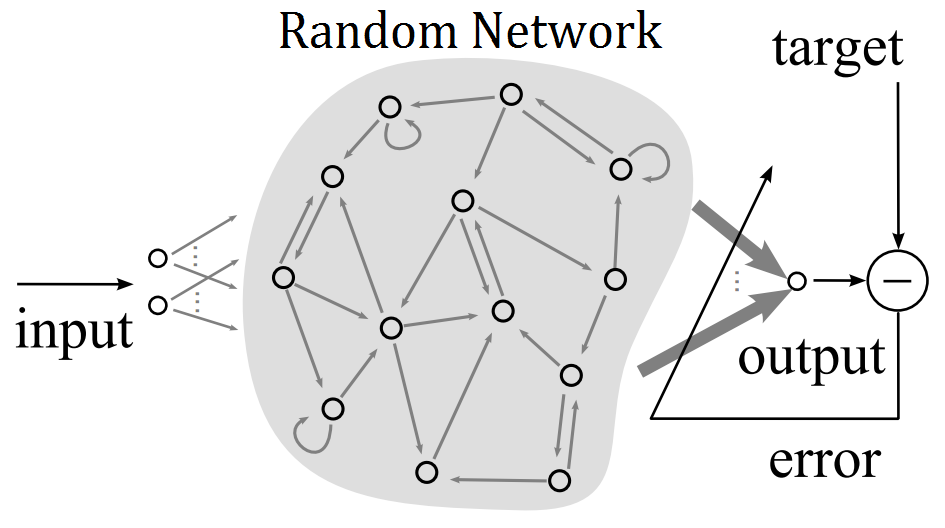
\includegraphics[width=0.9\linewidth]{fig2} }
%\caption2{\large In a reservoir network, only the weights in the output layer are trained by the errors. The network weights are {\em randomly} set at the beginning and never updated. }
\end{figure}
\large In a reservoir network, only the weights in the output layer are trained by the errors. The network weights and connections are \textbf {\em randomly} set at the beginning and never updated. Like conventional RNNs, a reservoir network possesses a {\em dynamical memory} and is able to process temporal context information.
\end{block}

\bigskip 

\begin{block}{\vspace{-13 mm} \LARGE Output Layer Training}
\large
Training the output layer is a common, non-temporal task of mapping the input to the target output. This is a well investigated domain in machine learning, and a large choice of methods are available. Some of the most popular are Linear Regression and SVMs.
\end{block}


\end{column}

\begin{column}{.45\linewidth}

\bigskip

\begin{block}{\vspace{-10 mm} \LARGE Reservoir Creation}
\large
However, not all reservoir networks with random architectures have desirable behavior. Most importantly, the cycles in the network can produce amplification effects, eventually saturating the nodes. \\
Good networks possess the following two useful, but conflicting, properties:\\
$\bullet$ Echo State Property: the effect of a previous state and input should vanish over time.\\
$\bullet$ Separability: different inputs should stabilize on different outputs. \\
\bigskip
A common practice to balance these two properties is to make the weight matrix {\em big, sparse and random}; which makes the activation signals {\em numerous, decoupled and varied}. The weight values are then downscaled to prevent any amplification.


\end{block}

\bigskip 

\begin{block}{\vspace{-13 mm} \LARGE A Toy Problem}
\large
We define a simple task to display the temporal memory of reservoir networks. The goal is to reproduce a random input signal with a K-steps delay.
\bigskip

\begin{figure}[t]
\fbox{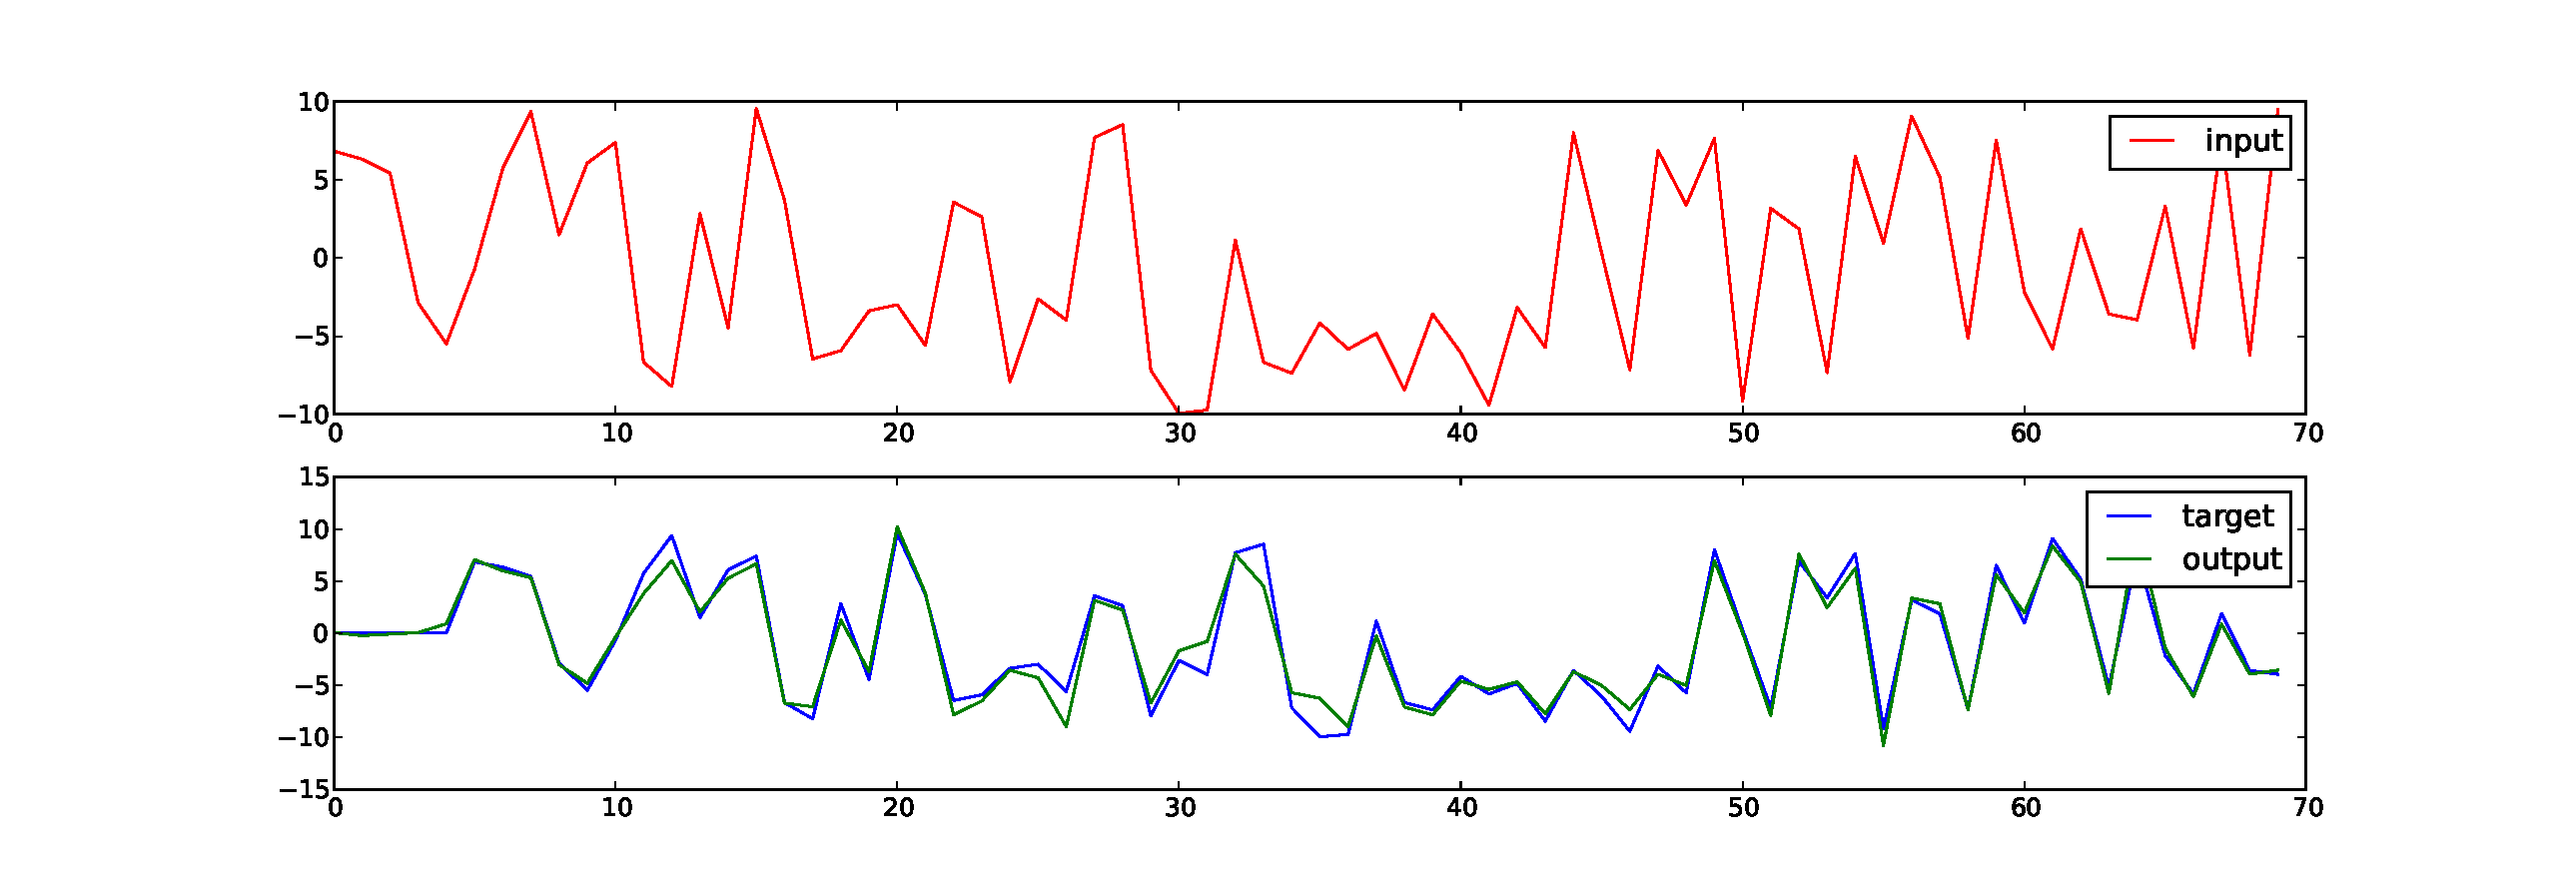
\includegraphics[trim=3cm 0 3cm 0, clip=true, width=0.9\linewidth]{fig3} }
\end{figure}
As shown above, a network consisting of just 50 neurons can reproduce the input signal (in red) with a 5 time-step delay almost perfectly. The desired target signal is in blue and the produced output signal in green.\\
\bigskip
\normalsize
$\ast$ Note: The above results are artificially worsened for visualization purposes.


\end{block}

\bigskip 

\begin{block}{\vspace{-13 mm} \LARGE Current Research and Applications}
\large 
Since it's inception in the early 2000s, the Reservoir Computing paradigm has been successfully been applied to a variety of scientific fields:\\
$\bullet$ NLP: {\em Phoneme recognition with large hierarchical reservoirs}, Triefenbach et al., NIPS 2011.\\
$\bullet$ Computational Neuroscience: {\em A reservoir of time constants for memory traces in cortical neurons}, Bernacchia et al., Nature Neuroscience 2011.\\
$\bullet$ Physics: {\em Constructing optimized binary masks for reservoir computing with delay systems}, Appeltant et al., Nature 2014\\
\bigskip
My own research is centering on two topics: applying the Reservoir Computing paradigm to speech NLP tasks within Pr. Rosenberg's lab; and studying how reservoir can be used for multi-task learning (as described by Collobert et al.), applying the paradigm to medical data under the supervision of Pr. Elhadad.

%add my own work
%multi task + NLP
%make pictures smaller

\end{block}

\end{column}


\end{columns}

\end{document}


%%%%%%%%%%%%%%%%%%%%%%%%%%%%%%%%%%%%%%%%%%%%%%%%%%%%%%%%%%%%%%%%%%%%%%%%%%%%%%%%%%%%%%%%%%%%%%%%%%%%
%%% Local Variables: 
%%% mode: latex
%%% TeX-PDF-mode: t